\section{Resultados}
\label{sec:resultados}

La validación se centró en comprobar que las operaciones cumplen sus
postcondiciones. Además de ejecutar los casos de prueba, se evaluó
directamente la postcondición de \texttt{buscarRutasDirectas} sobre el
resultado obtenido. La expresión evaluada devuelve \texttt{true}, lo que
confirma que todos los recorridos devueltos se encuentran dentro del
radio respecto del origen y del destino (Figura~\ref{fig:validacion}).

\begin{figure}[!t]
\centering
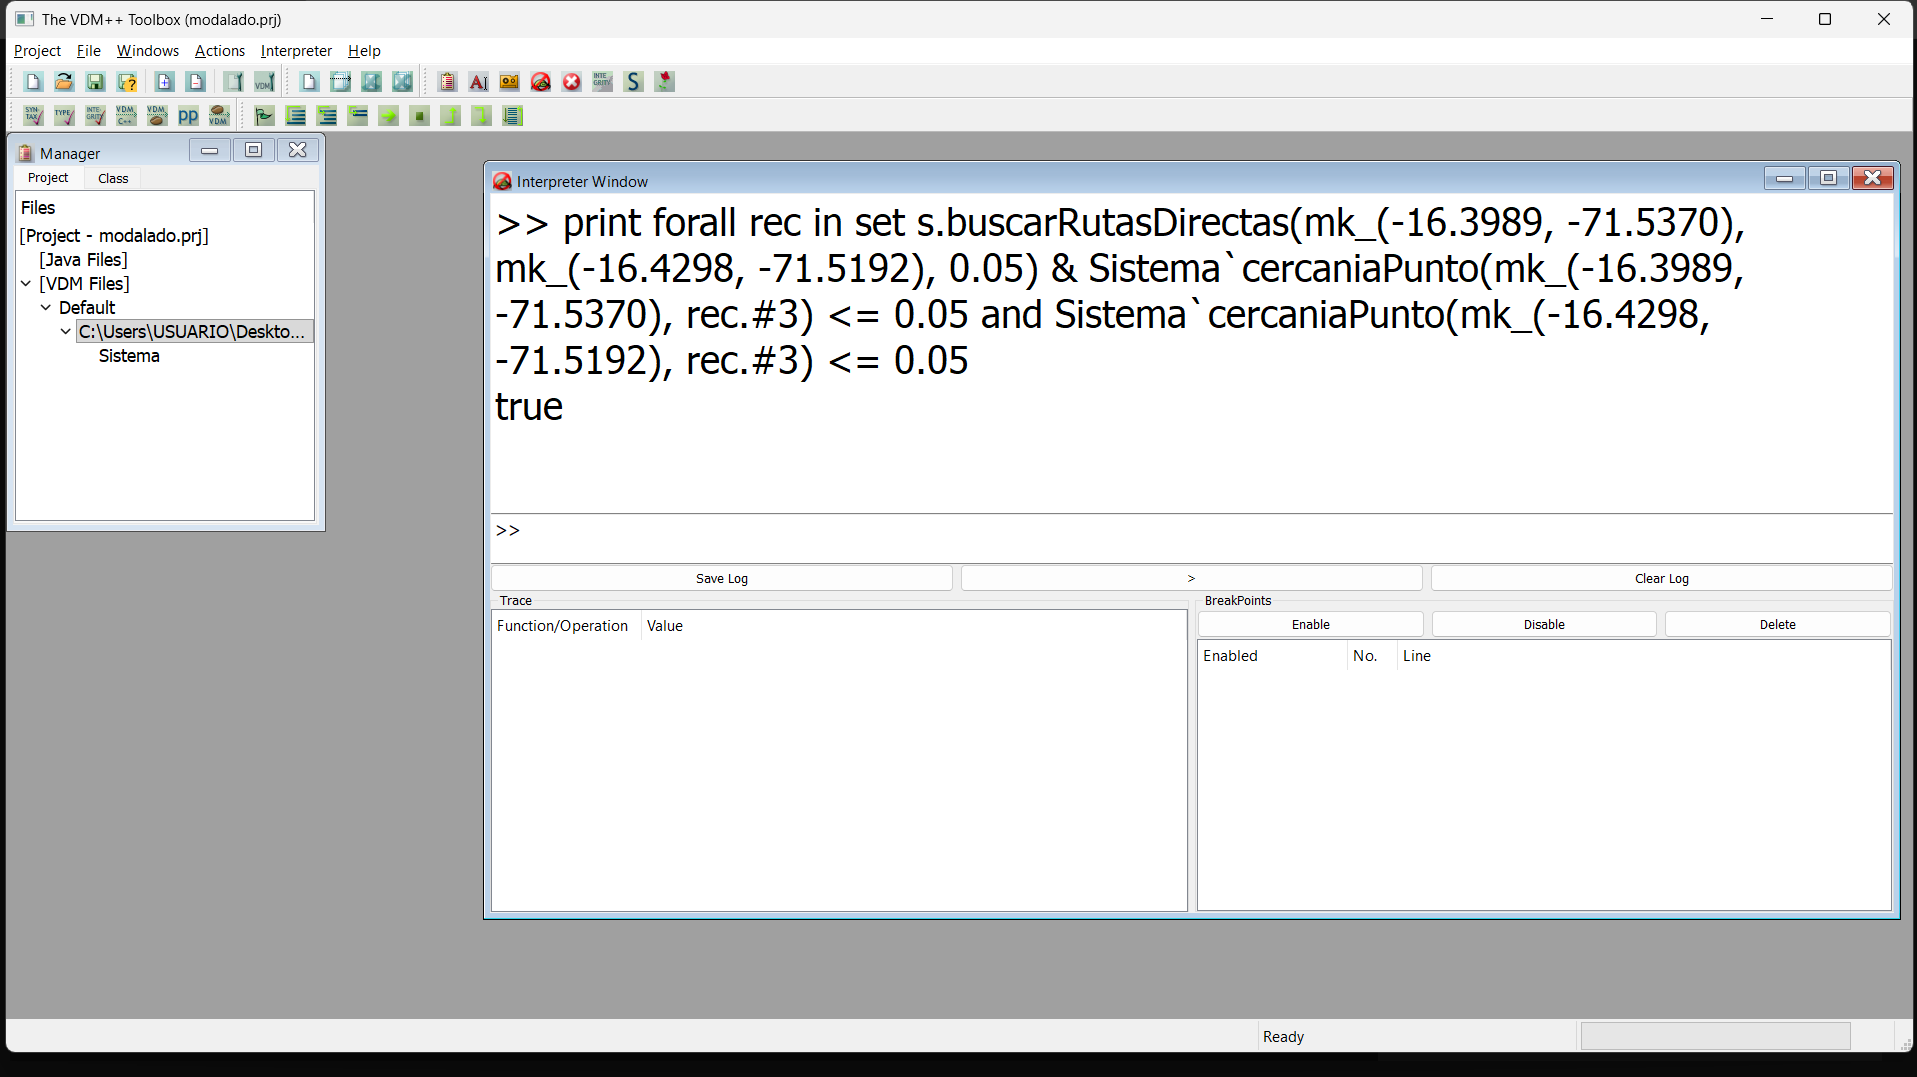
\includegraphics[width=\columnwidth]{images/Validacion_True.png}
\caption{Evaluación de la postcondición sobre el resultado: devuelve \texttt{true}.}
\label{fig:validacion}
\end{figure}

Adicionalmente, la Toolbox generó las obligaciones de prueba
(\emph{proof obligations}) asociadas a las postcondiciones de las
operaciones de búsqueda (Figura~\ref{fig:po}). Estas obligaciones
expresan formalmente las propiedades que el modelo debe satisfacer y
constituyen la base para una verificación deductiva más estricta.

\begin{figure}[!t]
\centering
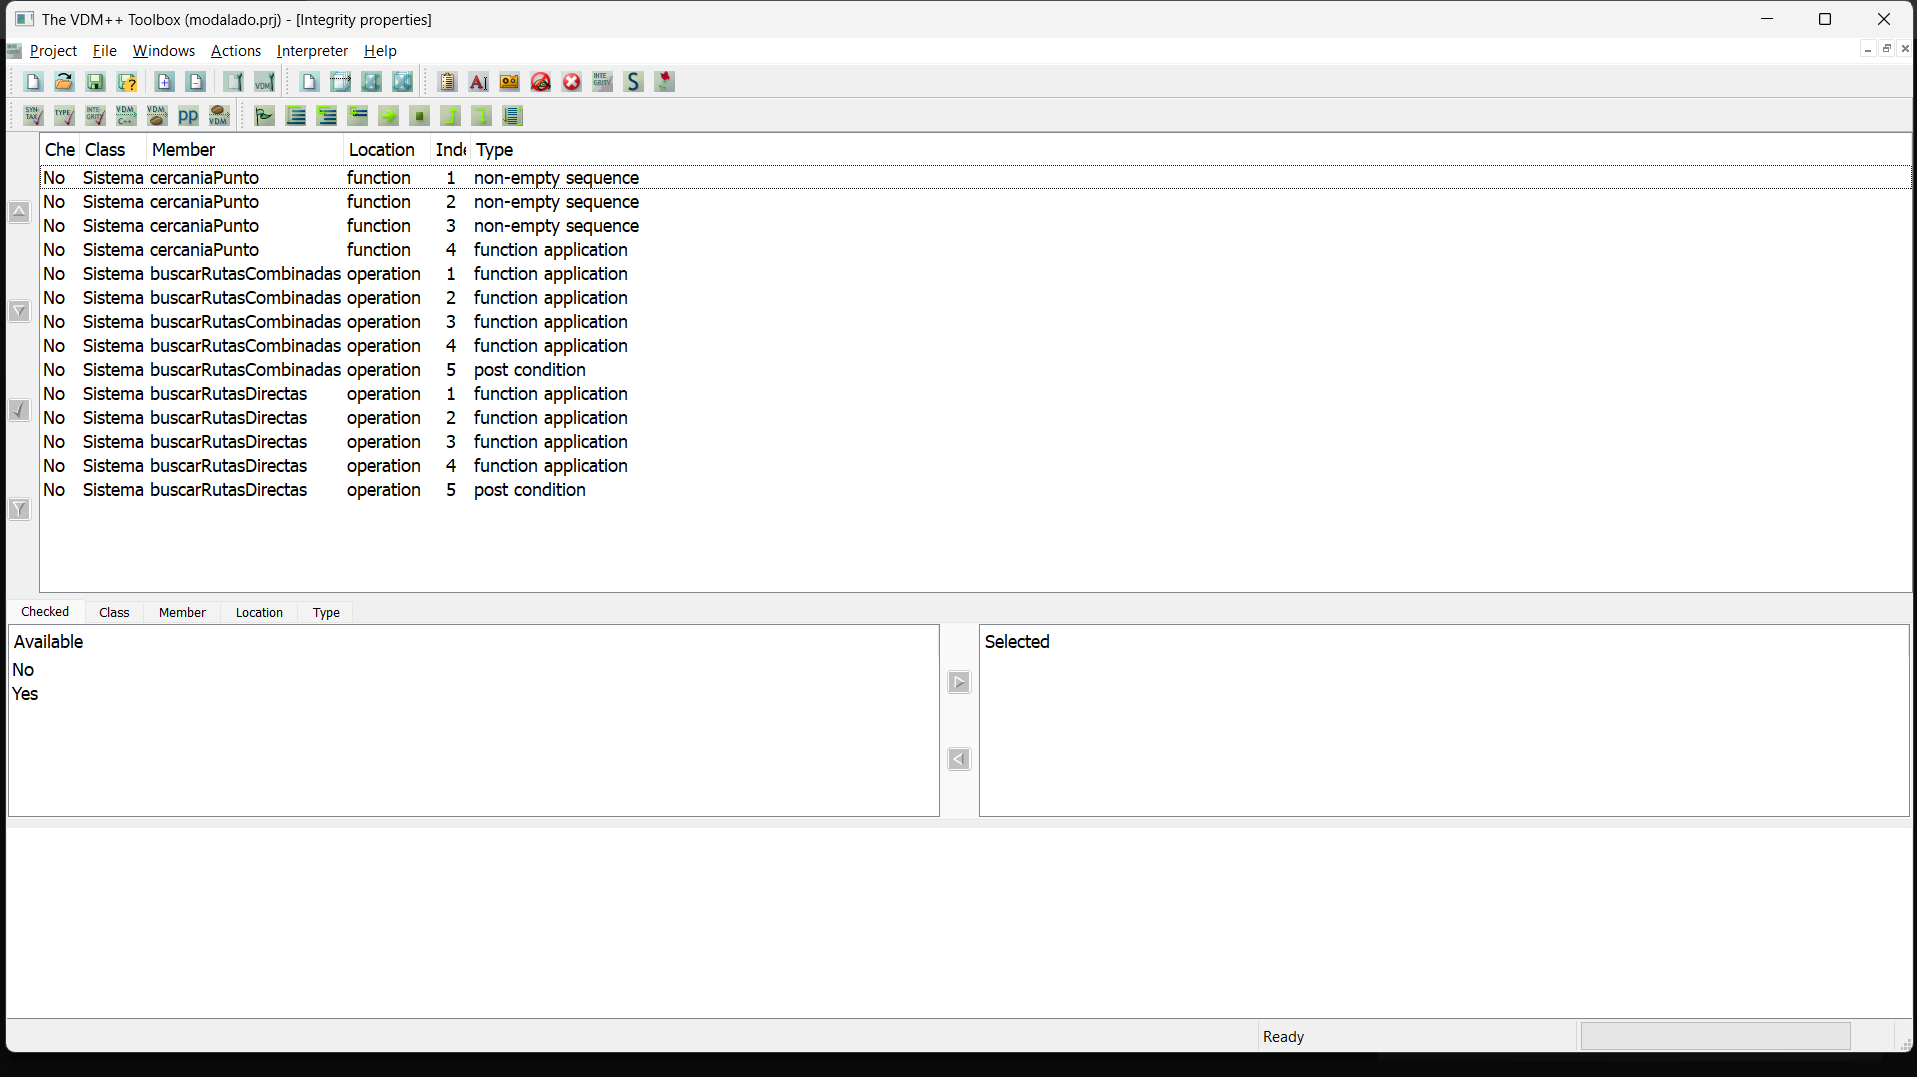
\includegraphics[width=\columnwidth]{images/Proof_Obligations.png}
\caption{Obligaciones de prueba generadas a partir de las postcondiciones.}
\label{fig:po}
\end{figure}
